\documentclass[tikz, border=10pt]{standalone}
%%%<
\usepackage{verbatim}
%%%>
\begin{comment}
:Title: Basic Philosophy concepts
:Tags: Diagrams;Graphs;Philosophy
:Author: Vilson Vieira
:Slug: philosophy

This graph diagram presents the basic Philosophy concepts of dialectics,
opposition and innovation.
\end{comment}
\tikzset{
    vertex/.style = {
        circle,
        fill            = black,
        outer sep = 2pt,
        inner sep = 1pt,
    }
}
\begin{document}
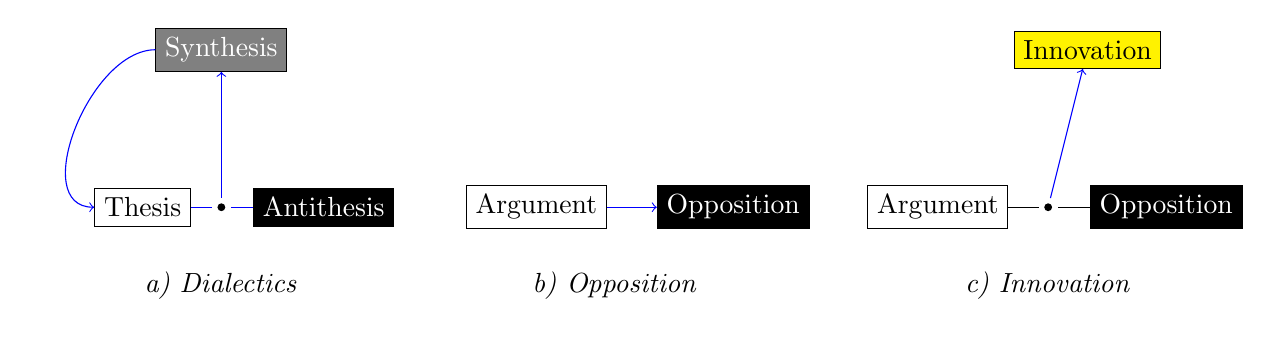
\begin{tikzpicture}
  % Dialectics
  \node[draw] (Thesis) at (0,0) {Thesis};
  \node[draw,fill=black,text=white] (Antithesis) at (2.3,0) {Antithesis};
  \node[draw,fill=gray,text=white] (Synthesis) at (1,2) {Synthesis};
  
  \draw node[vertex] (Joint) at (1,0) {};
  
  \draw[-,draw=blue] (Thesis) to (Joint);
  \draw[-,draw=blue] (Antithesis) to (Joint);
  \draw[->,draw=blue] (Joint) to (Synthesis);
  \draw[->,draw=blue] (Synthesis) to[in=180,out=180] (Thesis);
  
  \node at (1.0, -1.0) {\textit{a) Dialectics}};
  
  % Opposition
  \node[draw] (ArgumentA) at (5,0) {Argument};
  \node[draw,fill=black,text=white] (ArgumentB) at (7.5,0) {Opposition};
  
  \draw[->,draw=blue] (ArgumentA) to (ArgumentB);
  
  \node at (6., -1.0) {\textit{b) Opposition}};
  
  % Innovation
  \node[draw] (ArgumentA) at (10.1,0) {Argument};
  \node[draw,fill=black,text=white] (ArgumentB) at (13,0) {Opposition};
  \node[draw,fill=yellow] (ArgumentC) at (12,2) {Innovation};
  
  \draw node[vertex] (Joint) at (11.5,0) {};
  
  \draw[-] (ArgumentA) to (Joint);
  \draw[-] (ArgumentB) to (Joint);
  \draw[->,draw=blue] (Joint) to (ArgumentC);
  
  \node at (11.5, -1.0) {\textit{c) Innovation}};
\end{tikzpicture}
\end{document}